\documentclass[super,list,bibieee,myhdrone,table,math,chars]{cltart}
\graphicspath{{img/}}   % 设置图片所存放的目录
%\nofake
\begin{document}
\cltheading{cltart使用说明by\ cltian }
\clttitle{cltart使用说明}
\cltinfo{cltian\footnote{cltian个人主页:\url{http://github.com/foowaa/documentation}}——tianchunlin123@gmail.com}
\section{cltart文档类简介}
\par ``cltart''是为CTEX的article类定制的一个文档类,\emph{用于简化常见中文文档书写}。使用很简单:
\begin{verbatim}
\documentclass[arg1, arg2, ..., argN]{cltart}
\end{verbatim}
\par 具体的页面配置如下:
\begin{itemize}
  \item 使用A4页面,行间距1.5倍,段前段后0磅,section段前24磅、段后6磅,subsection段前12磅、段后6磅,subsection段前12磅、段后6磅
  \item 标题三号黑体加粗居中,信息五号黑体加粗居中,章节黑体小四黑体左顶格\footnote{请确定宋体、黑体、楷体和Times New Roman已安装。中文字体问题请参看《CTeX 宏集手册》。}
  \item 正文中文使用宋体小四,英文使用Times New Roman小四。
  \item 页眉页脚使用五号字
  \item caption段前6磅,段后0磅,使用五号字
  \item 参考文献提供GBT-7714和IEEE Trans格式,有中文建议使用GBT-7714格式。文档使用五号字,1.5倍行距
  \item 对浮动体进行设置,使之排版更紧密
\end{itemize}
\section{预定义命令和环境}
\par CTEX中默认使用黑体表示加粗,使用楷体表示斜体,这与Microsoft Word不同,cltart使用xeLaTex的AutoFakeBold和AutoFakeSlant加以设置,使之与Microsoft Word显示类似。如要取消此功能,即\smallblank{1}用黑体表示加粗,使用楷体表示斜体,在导言区使用\textbackslash nofake命令\footnote{详细的字体设置:\url{https://en.wikibooks.org/wiki/LaTeX/Fonts}和\url{https://github.com/wklchris/Note-by-LaTeX}}。如:
\begin{verbatim}
\documentclass[super,list,bibieee,myhdrone,table,math]{cltart}
\nofake
\begin{document}
...
...
\end{document}
\end{verbatim}

\blankline{1}

\par 关于文档开头的命令。cltart摒弃了LaTex内置的生成标题、作者、日期等的命令。自建命令完成这些功能,这些命令可写可不写,不写则无此信息。其中,\textbackslash clttitle{}命令和\textbackslash cltinfo{}命令请注意先后顺序。
\begin{itemize}
  \item \textbackslash clttitle{}命令,用在开头,生成标题。如果不写则无标题。
  \item \textbackslash cltinfo{}命令,用在开头,生成相关信息(如作者,联系方式,日期等)。如果不写则无信息。
  \item \textbackslash cltheading{}命令,用在开头,如传入myhdrone, myhdrtwo,则必须设置,其为页眉信息。请参看节-\ref{sec3}。
\end{itemize}
\par 如本文开头是这样写的:
\begin{verbatim}
\documentclass[super,list,bibieee,myhdrone,table,math]{cltart}
\begin{document}
\cltheading{cltart使用说明by\ cltian}
\clttitle{cltart使用说明}
\cltinfo{cltian——tianchunlin123@gmail.com}
...
...
\end{document}
\end{verbatim}

\blankline{1}

\par 便捷的空格、换行、换页命令:
\begin{itemize}
  \item \textbackslash smallblank{},可传入参数N,会生成N个1/3em的空格。
  \item \textbackslash bigblank{},可传入参数N,会生成N个1em的空格。
  \item \textbackslash nextline{},可传入参数N,会生换行N次,换行之后文字不缩进。(适用于文字之间)
  \item \textbackslash nextlineindent{},可传入参数N,会生换行N次,换行之后文字缩进。(适用于文字之间)
  \item \textbackslash blankline{},可传入参数N,会产生N个空白行。(适用于不同元素之间)
  \item \textbackslash blankpage{},可传入参数N,另起一页,并生成N个空白页。
  \item \textbackslash nextpage,无参数,另起一页。
\end{itemize}

\blankline{1}

\par 在传入list参数后,可以使用预设的文字带颜色框。\textbackslash boxone\boxone{这是boxone},\textbackslash boxtwo\boxtwo{这是boxtwo},\textbackslash boxthree \boxthree{这是boxthree}\footnote{更多的定义方法参见tcolorbox包}。

\blankline{1}
\par 预定义\textbackslash famousqoute{}{}命令,此命令有2个参数,其中第一个参数表示名人的姓名,第二个参数表示出处。例如:
\nextpage
\begin{famousquote}{陶渊明}{《归去来兮辞》}
归去来兮,田园将芜胡不归。既自以心为形役,奚惆怅而独悲。悟已往之不谏,知来者之可追。识迷途其未远,觉今是而昨非。
\end{famousquote}
\section{参考文献选项}
\par 如果要使用参考文献,请\textbf{务必}传入参数<numbers|super|authoryar>,如要使用IEEE Trans参考文献格式,使用参数bibieee,否则默认使用GBT-7714。传递参数方法如下,之后不再赘述。
\begin{verbatim}
\documentclass[super,bibieee]{cltart}
\end{verbatim}
\subsection{引用格式}\label{1.1}
\begin{itemize}
  \item numbers:[1]
  \item super:上标 [1]
  \item authoryear:(Jones, 1995)
\end{itemize}
\par 引用使用\textbackslash cite{},例如\smallblank{1}如文献\cite{tian2017deep,yuan2018auxiliary}。如要在super中使用numbers,使用命令\textbackslash citens{},例如\smallblank{1}如文献\citens{tian2017deep,yuan2018auxiliary}
\subsection{参考文献格式}
\par 默认使用GBT-7714格式,如想使用IEEE Trans格式,请传入bibieee参数。注意:IEEE Trans格式比较适用于参考文献为英文论文,否则不要使用。
\section{页眉页脚}\label{sec3}
采用fancyhdr包,我们预定义了6种页眉页脚格式,分别为:myhdrone,myhdrtwo,myhdrthree,myhdrfour,myhdrfive和默认,不设置即为默认格式。
\begin{itemize}
  \item myhdrone——必须设置\textbackslash cltheading{},页眉左侧为\textbackslash cltheading{}的内容,右侧为页码。
  \item myhdrtwo——必须设置\textbackslash cltheading{},页眉居中为\textbackslash cltheading{}的内容,页脚居中为页码。
  \item myhdrthree——页眉左侧为章节号和章节标题,右侧为页码。
  \item myhdrfour——页眉居中为章节号和章节标题,页脚居中为页码。
  \item myhdrfive——页眉页脚为空。
  \item 默认——页眉为空,页脚居中为页码。
\end{itemize}
\section{杂项}
\par \textbf{list}。引入verbatim,listings,tcolorbox,salgpseudocode,algorithm,algorithmicx包,并进行了一些配置,可以支持verbatim,源代码和伪代码。源代码如下:
\begin{lstlisting}[language=c++]
typedef struct ImageData {
  ImageData() {
    data = nullptr;
    width = 0;
    height = 0;
    num_channels = 0;
  }

  ImageData(int32_t img_width, int32_t img_height,
    int32_t img_num_channels = 1) {
    data = nullptr;
    width = img_width;
    height = img_height;
    num_channels = img_num_channels;
  }

  uint8_t* data;
  int32_t width;
  int32_t height;
  int32_t num_channels;
} ImageData;

  typedef struct {
    double x;
    double y;
  } FacialLandmark;

    uint8_t* data;
  int32_t width;
  int32_t height;
  int32_t num_channels;
} ImageData;

  typedef struct {
    double x;
    double y;
  } FacialLandmark;
}
\end{lstlisting}
\par \textbf{math}。引入了amsmath,mathtools,amsfonts,amssymb,mathdots,mathrsfs,yhmath,esint,extarrows包方便高级数学公式书写。例如:
\nextline{1}

Pascal’s rule is
\[
\binom{n}{k} =\binom{n-1}{k}
+ \binom{n-1}{k-1}
\]

\par \textbf{color}。引入了xcolor包\footnote{具体使用参见\url{https://en.wikibooks.org/wiki/LaTeX/Colors}}。传入color参数相当于:
\begin{verbatim}
\usepackage[usenames,dvipsnames,table]{xcolor}
\end{verbatim}

\par \textbf{table}。引入了ctable,longtable,multirow,array,booktabs包,方便进行复杂表格设计。例子如表-\ref{table1}。

\ctable[cap = {TABLE CAPTION},caption = {例子}, label={table1}]{cc}
{
  % You specify table footnotes here.
  \tnote[$\ast$]{DA FOOTNOTE 1}
  \tnote[$\dagger$]{dat other footnote}
  \tnote[b]{mistakes are possible (you must match these up yourself)}
}{
\FL % FLORIDA (just kidding, means "first line")
COL 1\tmark[a] & COL 2\tmark[$\ast$]
\ML % middle line
6.920e+00\tmark[$\dagger$]     &   0.09781\\
97     &   2000
\LL % last line
}

\par \textbf{nohref}。如传入nohref参数,则不使用超链接。默认使用超链接\footnote{具体参看\url{https://en.wikibooks.org/wiki/LaTeX/Hyperlinks}}。

\par \textbf{geometry}。引入geomrtry包调整页面。

\par \textbf{tikz}。引入tikz包绘图\footnote{使用见:\url{https://en.wikibooks.org/wiki/LaTeX/PGF/TikZ}}。

\par \textbf{syntaxonly}。引入syntonly包,进行语法检查且不生成pdf文件(往往这样会更快编译),此选项比较适合于确认文档有无语法错误。

\par \textbf{chars}。引入textcomp,pifont,ifsym包,以使用特殊符号\footnote{详情使用见\url{https://people.math.osu.edu/snapp.14/immerse/symbolList.pdf}和\nextline{1} \url{https://en.wikibooks.org/wiki/LaTeX/Special_Characters}}。例如30 \textcelsius{},200 \textcentoldstyle,10000 \textyen,\ding{85},\FilledSquareShadowC,\LongPulseLow,\textifsym{mm<DDD>mm},\textifsym{-123.456},\SnowCloud,\Taschenuhr,\Letter

\begin{figure}[htbp]
    \centering
    \begin{subfigure}[htbp]{0.17\textwidth}
        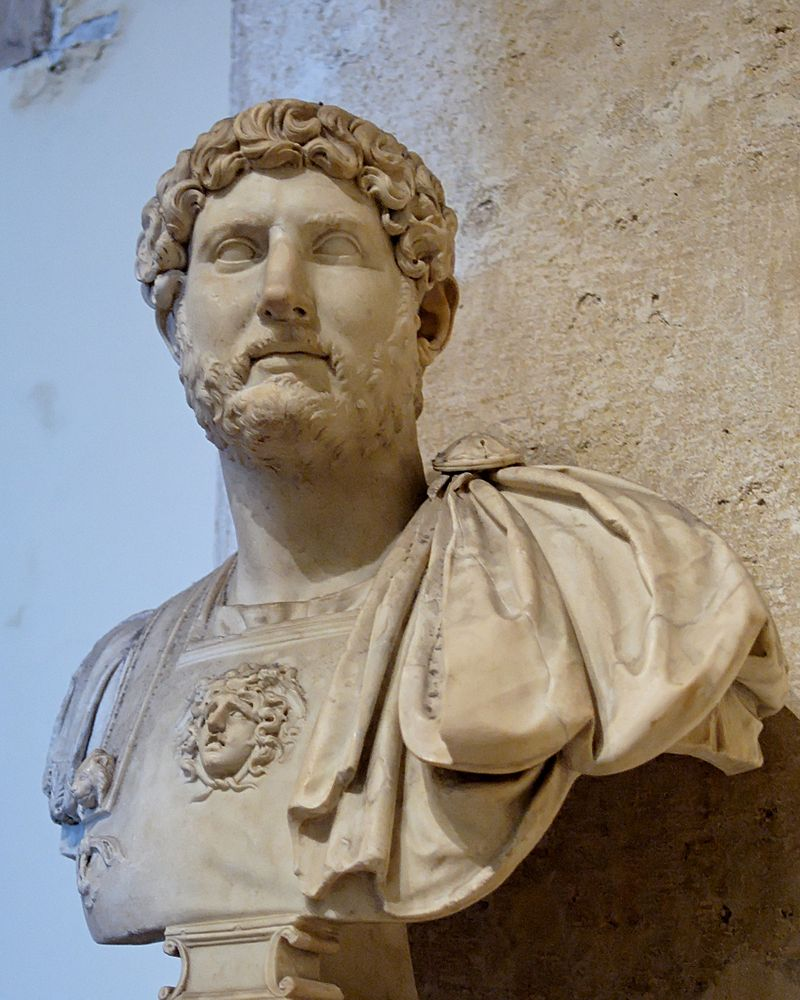
\includegraphics[width=\textwidth]{Hadrian.jpg}
        \caption{Hadrian}
        \label{fig:Hadrian}
    \end{subfigure}
    ~ %add desired spacing between images, e. g. ~, \quad, \qquad, \hfill etc.
      %(or a blank line to force the subfigure onto a new line)
    \begin{subfigure}[htbp]{0.17\textwidth}
        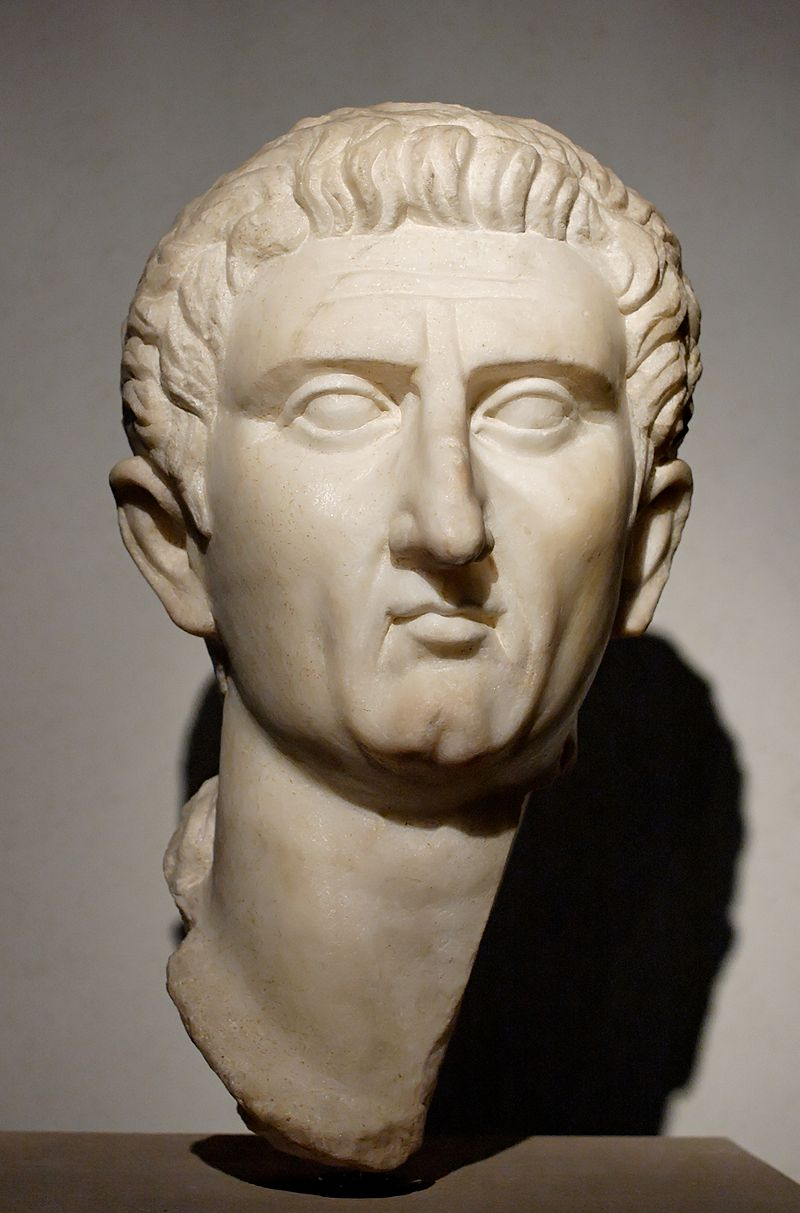
\includegraphics[width=\textwidth]{Nerva.jpg}
        \caption{Nerva}
        \label{fig:Nerva}
    \end{subfigure}
    ~ %add desired spacing between images, e. g. ~, \quad, \qquad, \hfill etc.
    %(or a blank line to force the subfigure onto a new line)
    \begin{subfigure}[htbp]{0.17\textwidth}
        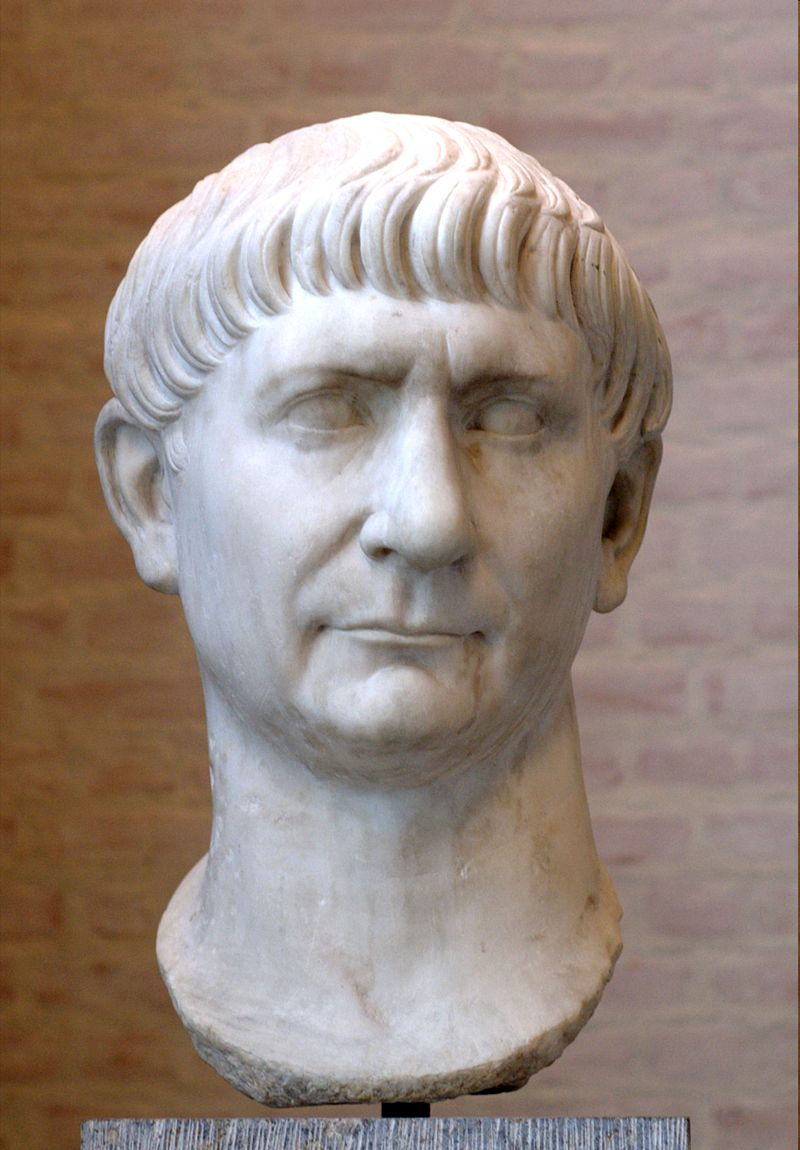
\includegraphics[width=\textwidth]{Traianus.jpg}
        \caption{Traianus}
        \label{fig:Traianus}
    \end{subfigure}
    \caption{罗马帝国帝王}\label{fig:roman}
\end{figure}

\par \textbf{图片}。默认导入graphicx,subcaption,bicaption,float包,并进行了图片样式的调整,可以使用子图和双语图。\footnote{详情使用见\url{https://en.wikibooks.org/wiki/LaTeX/Importing_Graphics}和\nextline{1} \url{https://en.wikibooks.org/wiki/LaTeX/Floats,_Figures_and_Captions}}。





\bibliography{bib/ref}
\end{document}
